\documentclass{bioinfo}
\copyrightyear{2013}
\pubyear{2013}
%\usepackage[top=1in, bottom=1in,right=1in,left=1in]{geometry}                % See geometry.pdf to learn the layout options. There are lots.
%\geometry{letterpaper}                   % ... or a4paper or a5paper or ... 
%\geometry{landscape}                % Activate for for rotated page geometry
%\usepackage[parfill]{parskip}    % Activate to begin paragraphs with an empty line rather than an indent
%\usepackage[utf8]{inputenc}
\usepackage{graphicx}
\usepackage{amssymb}
\usepackage{amsmath}
\usepackage{amsthm} %pour les newtheorem
\usepackage{epstopdf}
\usepackage{framed}
\usepackage{xspace}
%\usepackage{tcolorbox}
\usepackage{relsize}
%\usepackage{natbib}
\usepackage[colorinlistoftodos]{todonotes}

\usepackage{soul}

\colorlet{shadecolor}{yellow!80!orange!50}
\sethlcolor{shadecolor}
\makeatletter

\renewenvironment{snugshade}{%
 \def\FrameCommand##1{\hskip\@totalleftmargin \hskip-\fboxsep
 \colorbox{shadecolor}{##1}\hskip-\fboxsep
     % There is no \@totalrightmargin, so:
     \hskip-\linewidth \hskip-\@totalleftmargin \hskip\columnwidth}%
 \MakeFramed {\advance\hsize-\width
   \@totalleftmargin\z@ \linewidth\hsize
   \@setminipage}}%
 {\par\unskip\endMakeFramed}

\makeatother

\newcommand{\highlight}[1]{{\begin{snugshade}{#1}\end{snugshade}}}

%\usepackage{subfig} %Subfigures
\usepackage{subcaption} %Subfigures

\usepackage{tikz}
\usepackage{amsmath}
\usepackage{ifthen}
\usepackage{relsize}
\usepackage{multirow}
\usepackage{cleveref}
\usepackage{url}

\usetikzlibrary{positioning}
\usetikzlibrary{matrix}
\usetikzlibrary{calc}
\usetikzlibrary{shapes}
\usetikzlibrary{arrows}
\usetikzlibrary{fit}
\usetikzlibrary{decorations}
\usetikzlibrary{snakes}
\usetikzlibrary{shadows}
\pgfdeclarelayer{background}
\pgfdeclarelayer{backbackground}
\pgfdeclarelayer{foreground}
\pgfsetlayers{backbackground,background,main,foreground}

\usepackage[noend,ruled,vlined]{algorithm2e}

\newtheorem{theorem}{Theorem}[section]
\newtheorem{lemma}[theorem]{Lemma}
\newtheorem{proposition}[theorem]{Proposition}
\newtheorem{corollary}[theorem]{Corollary}
\newtheorem{description}{Description}

\crefmultiformat{equation}{Equations~(#2#1#3)}%
{ and~(#2#1#3)}{, (#2#1#3)}{ and~(#2#1#3)}


%\usepackage[applemac]{inputenc} %for the encoding 




\newcommand{\RNAmutants}{\texttt{RNAmutants}\xspace}
\newcommand{\RNApyro}{\texttt{RNApyro}\xspace}
\newcommand{\RNAinverse}{\texttt{RNAinverse}\xspace}
\newcommand{\RNASSD}{\texttt{RNA-SSD}\xspace}
\newcommand{\INFORNA}{\texttt{INFO-RNA}\xspace}
\newcommand{\NUPACK}{\texttt{NUPACK:Design}\xspace}
\newcommand{\RNAiFOLD}{\texttt{RNAiFOLD}\xspace}
\newcommand{\frankenstein}{\texttt{Frnakenstein}\xspace}
\newcommand{\RNAexinv}{\texttt{RNAexinv}\xspace}
\newcommand{\rnaDesign}{\texttt{rnaDesign}\xspace}
\newcommand{\RNAensign}{\texttt{RNA-ensign}\xspace}
\newcommand{\GC}{\Gb\Cb}
\newcommand{\GCContent}{\Gb\Cb-content\xspace}
\newcommand{\SFold}{\texttt{SFold}\xspace}

\newcommand{\ourprog}{\texttt{IncaRNAtion}\xspace} 

\newcommand{\red}[1]{{\color{red}#1}}
\newcommand{\farna}{\texttt{FARNA}\xspace}
\newcommand{\mcfoldmcsym}{\texttt{MC-Pipeline}\xspace}
\newcommand{\mcfold}{\texttt{MC-Fold}\xspace}
\newcommand{\mcsym}{\texttt{MC-Sym}\xspace}
\newcommand{\nast}{\texttt{NAST}\xspace}
\newcommand{\ifoldrna}{\texttt{iFoldRNA}\xspace}
\newcommand{\rnafold}{\texttt{RNAfold}\xspace}
\newcommand{\rnasubopt}{\texttt{RNAsubopt}\xspace}
\newcommand{\rnawolf}{\texttt{RNAwolf}\xspace}
\newcommand{\rnastructure}{\texttt{RNAstructure}\xspace}
\newcommand{\contrafold}{\texttt{contrafold}\xspace}
\newcommand{\unafold}{\texttt{unafold}\xspace}
\newcommand{\rnadd}{\texttt{RNA2D3D}\xspace}
\newcommand{\assemble}{\texttt{assemble}\xspace}
\newcommand{\fred}{\texttt{FR3D}\xspace}
\newcommand{\rnajunction}{\texttt{RNAjunction}\xspace}
\newcommand{\rnamotif}{\texttt{RNAmotif}\xspace}
\newcommand{\treefolder}{\texttt{TreeFolder}\xspace}
\newcommand{\barnacle}{\texttt{BARNACLE}\xspace}
\newcommand{\contextfold}{\texttt{contextfold}\xspace}

\newcommand{\RNASTRAND}{{\sf RNA STRAND}\xspace}

%\newcommand{\citep}{\cite}
\newcommand{\Z}[2]{\mathcal{Z}{\substack{[#2]\\#1}}}
\newcommand{\B}{\mathcal{B}}
\newcommand{\Kron}{\delta}
\newcommand{\ub}{\bullet}
\newcommand{\op}{\texttt{(}}
\newcommand{\cp}{\texttt{)}}

\newcommand{\Ab}{{\sf{A}}\xspace}
\newcommand{\Cb}{{\sf{C}}\xspace}
\newcommand{\Gb}{{\sf{G}}\xspace}
\newcommand{\Ub}{{\sf{U}}\xspace}

\newcommand{\gc}{{\#\text{{\sf gc}}}}
\newcommand{\PE}[1]{E(#1)}
\newcommand{\EI}{\text{EI}}
\newcommand{\ES}{{{E}}}
\newcommand{\ISO}{\text{ISO}}
\newcommand{\Prob}{\mathbb{P}}
\newcommand{\Target}{{S}^*}
\newcommand{\Struct}{{S}}
\newcommand{\N}{{N}}
\newcommand{\CNBP}[1]{\gamma(#1)}
\newcommand{\BoolTrue}{{\sf T}}
\newcommand{\BoolFalse}{{\sf F}}

\newcommand{\CFramed}[2][gray]{\begin{tcolorbox}[colframe=#1,title=To be included only if space allows\ldots,colback=white]#1\end{tcolorbox}}
\renewcommand{\CFramed}[2][gray]{}

\newcommand{\oururl}{\url{http://csb.cs.mcgill.ca/incarnation/}}


\begin{document}
\firstpage{1}

\title{A weighted sampling algorithm for the design of RNA sequences with targeted secondary structure and nucleotides distribution}
\author{Vladimir Reinharz$^1$, Yann Ponty$^{2,*}$, J\'er\^{o}me Waldisp\"{u}hl$^{1}$\footnote{to whom correspondence should be addressed}}
\address{$^1$ School of Computer Science, McGill University, Montreal, Canada\\ $^2$ Laboratoire d'informatique, \'Ecole Polytechnique, Palaiseau, France.}

\history{Received on XXXXX; revised on XXXXX; accepted on XXXXX}

\editor{Associate Editor: XXXXXXX}

\maketitle
%\section{}
%\subsection{}
\begin{abstract}
\section{Motivations:} The design of RNA sequences folding into predefined secondary structures is a milestone for many synthetic biology and gene therapy studies. Most of the current software uses similar local search strategies (i.e. a random seed is progressively adapted to acquire the desired folding properties) and more importantly do not allow the user to control explicitly the nucleotide distribution such as the \GCContent in their sequences. However, the latter is an important criterion for large-scale applications as it could presumably be used to design sequences with better transcription rates and/or structural plasticity.

\section{Results:}
In this paper, we introduce \ourprog, a novel algorithm to design RNA sequences folding into target secondary structures with a predefined nucleotide distribution.  \ourprog uses a global sampling approach and weighted sampling techniques. We show that our approach is fast (i.e. running time comparable or better than local search methods), seed-less (we remove the bias of the seed in local search heuristics), and successfully generates high-quality sequences (i.e. thermodynamically stable) for any \GCContent. To complete this study, we develop an hybrid method combining our global sampling approach with local search strategies. Remarkably, our glocal methodology overcomes both local and global approaches  for sampling sequences with a specific GC content and target structure.
\section{Availability:} 
\ourprog is available at \href{http:// csb.cs.mcgill.ca/incarnation/}{csb.cs.mcgill.ca/incarnation/}
\section{Contact:} \href{jeromew@cs.mcgill.ca}{jeromew@cs.mcgill.ca}, \href{yann.ponty@lix.polytechnique.fr}{yann.ponty@lix.polytechnique.fr}\\
\noindent
\textbf{Key words:} RNA, secondary structure, design, weighted sampling, GC-content.
\end{abstract}


%!TEX root = main_ISMB.tex
\section{Introduction}
\label{sec:introduction}

At the core of the emerging field of synthetic biology resides our capacity to design and re-engineer molecules with target functions. RNA molecules are well tailored for such applications. The ease to synthesize them (they are directly transcribed from DNA) and the broad diversity of catalytic and regulation functions they can perform enable to integrate \textit{de-novo} logic  circuits within living cells \cite{Rodrigo:2012fk} or re-program existing regulation mechanisms \cite{Chang:2012uq}. Future advances and applications of these techniques in gene-therapy studies will strongly rely on efficient computational methods to design and re-engineer RNA molecules.

Most of RNA functions are, at least partially, encoded by the three-dimensional molecular structures, which are themselves primarily determined by the secondary structures. The development of efficient algorithms for designing RNA sequences with pre-defined secondary structures is thus a milestone to enter the synthetic biology era. \RNAinverse pioneered RNA secondary structure design algorithms. It has been developed and distributed with the Vienna RNA package \cite{Hofacker:1994}. However, only posterior experimental studies revealed the potential and practical impact of these techniques. Thereby, during the last 6 years many improvements and variants of \RNAinverse have been proposed. Conceptually, almost all of existing algorithms follow the same approach. First a seed sequence is selected, then a local search strategy is used to mutate the seed and find, in its vicinity, a sequence with desired folding properties. Using this strategy, \INFORNA \cite{Busch:2006uq}, \RNASSD \cite{Aguirre-Hernandez:2007kx} and \NUPACK \cite{Zadeh:2011fk} significantly improved the performance of RNA secondary structure design algorithms. More recent research studies aimed to include more constraints in the selection criteria. \RNAexinv focused on the design of sequences with enhanced thermodynamical and mutational robustness \cite{Avihoo:2011fk}, while \frankenstein enables to design RNA with multiple target structures \cite{Lyngso:2012vn}.

We recently introduced with \RNAensign a novel paradigm for the search strategy of RNA secondary structure design algorithm \cite{Levin:2012kx}. Instead of a local search approach, we proposed a global sampling strategy of the mutational landscape based on the \RNAmutants algorithm~\cite{Waldispuhl2008}. This methodology offered promising performances, but suffered from  prohibitive runtime and memory consumption. Following our work, Garcia-Martin and co-workers proposed \RNAiFOLD, an alternate methodology that uses constraint programming techniques to prune the mutational landscape. While also suffering from prohibitive running times, it is worth noting that this latter algorithm also proposes a seed-less approach to the RNA secondary structure design problem.

In this paper, we introduce \ourprog, a RNA secondary structure design algorithm that benefits of our recent algorithmic advances \cite{Reinharz:2013aa} to expand our original \RNAensign algorithm \cite{Levin:2012kx}. \ourprog addresses previous limitations of \RNAensign and offers new functionalities. First, while our previous program had a running time complexity of $\mathcal{O}(n^5)$, \ourprog now runs in linear-time and space complexity, allowing it to demonstrate similar speeds as any local search algorithm. Next, \ourprog is \textit{seed-less}. Unlike \RNAensign, it does not require a seed sequence to initiate its search. Finally, \ourprog implements a novel algorithm using weighted sampling techniques~\cite{Bodini2010} that enables us to control, for the first time, \textit{explicitly} the \GCContent of the solution. This functionality is essential because wild-type sequences within living organisms often present medium or low \GCContent, presumably to offer better transcription rates and/or structural plasticity. Previous programs do not allow to control this parameter and tend to output sequences with high \GCContent{}s. 

We demonstrate the performance of our algorithms on a set of real RNA structures extracted from the \RNASTRAND database \cite{andronescu2008rna}. To complete this study, we develop an hybrid method combining our global sampling approach with local search strategies such as the one implemented in \RNAinverse.  Remarkably, our glocal methodology overcomes both local and global approaches  for sampling sequences with a specific GC content and target structure.

%!TEX root = main_ISMB.tex
\section{Methods}
\label{sec:methods}



We introduce a probabilistic model for the design of RNA sequences with a specific \GCContent and folding into a predefined secondary structure.
For the sake of simplicity, we choose to base this proof-of-concept implementation on a simplified free-energy function $\ES(\cdot)$, which only considers the contributions of 
stacked canonical base-pairs. We show how a modification of the dynamic programming scheme used in \RNAmutants allows for the sampling of good and diverse design candidates, in linear time and space complexities.


%To that purpose, a Boltzmann weighted distribution is used, based on a pseudo-energy function $\PE{\cdot}$ which includes contributions for both the free-energy and its putative isostericity towards a multiple sequence alignment. In this model, the probability that the nucleotide at a given position needs to be mutated (i.e. corresponds to a sequencing error) can be computed using a variant of the \emph{Inside-Outside algorithm}~\cite{Lari1990}.
%
%\subsection{Probabilistic model}
%Let $\Omega$ be an gap-free RNA alignment sequence, $S$ its associated secondary structure, 
%then any sequence $s$ is assigned a probability proportional to its Boltzmann factor
%\begin{align*}
%  \mathcal{B}(s) &= e^\frac{-\PE{s}}{RT}, &&\text{with}&\PE{s}&:=\alpha\cdot\ES(s,S)+(1-\alpha)\cdot\EI(s,S,\Omega),
%\end{align*}
%where $R$ is the Boltzmann constant, $T$ the temperature in Kelvin, $\ES(s)$ and $\EI(s,S,\Omega)$ 
%are the free-energy and isostericity contributions respectively (further described below), and $\alpha\in[0,1]$ is an arbitrary parameter that sets the relative weight for both contributions.
%
%\subsubsection{Energy contribution}
\subsection{Definitions}

A targeted secondary structure $\Target$ is given as a non-crossing arc-annotated sequence,  where 
$\Target_i$ stands for the base-pairing position of position $i$ in $\Target$ if any (and, reciprocally, $\Target_{\Target_i}=i$), or $-1$ otherwise. 
In addition, we denote by $\gc(s)$ the number of occurrences of \Gb and \Cb in an RNA sequence $s$.

\subsubsection{Simplified energy model}
We use a simplified free-energy model which only includes additive contributions from stacking base-pairs. Using individual values from the Turner 2004 model (retrieved from the NNDB~\cite{Turner2010}). Given a candidate sequence $s$ for a secondary structure $S$, the free-energy of $S$ on $s$ is given by
\begin{align*}
  \ES(s,S) = \sum_{\substack{(i,j)\to (i',j')\in S\\ \text{stacking pairs}}}\ES^{\beta}_{s_is_j\to s_{i'}s_{j'}} 
\end{align*}
where $\ES^{\beta}_{ab\to a'b'}$ is set to $0$ if $ab=\varnothing$ (no base-pair to stack onto), the tabulated free-energy of stacking pairs $(ab)/(a'b')$ in the Turner model if available, or $\beta\in[0,\infty]$ for non-Watson-Crick/Wobble pairs (i.e. not in $\{\Gb\Ub,\Ub\Gb,\Cb\Gb,\Gb\Cb, \Ab\Ub\text{ or }\Ub\Ab\}$). This latter parameter allows one to choose whether to simply penalize invalid base pairs ($\beta>0$), or forbid them altogether ($\beta = +\infty$).

\subsubsection{\GCContent weighted pseudo-Boltzmann ensemble and distribution}

In order to counterbalance the documented tendency of sampling methods to generate \Gb\Cb-rich sequences~\cite{Levin:2012kx}, we introduce a parameter $x\in\mathbb{R}^+$, whose value will influence the \GCContent of generated sequences. Let $\Target$ be a targeted secondary structure, then let us define the pseudo-Boltzmann factor $\B_{x}(s,S)$ of a sequence $s$ such that
\begin{equation}
\B_{x, \Target}(s) = e^{\frac{-\ES(s,\Target)}{RT}}\cdot x^{\gc(s)}
\label{def:genBoltz}
\end{equation}
where $R$ is the Boltzmann constant and $T$ the temperature in Kelvin.

Summing the pseudo-Boltzmann factor over all possible sequences of a given length $|\Target|$, one obtains the pseudo-partition function $\mathcal{Z}_{x,\Target}$, from which one defines the pseudo-Boltzmann probability $\Prob_{x,\Target}(s)$ of each sequence $s$, respectively such that 
\begin{align}\mathcal{Z}_{x,\Target} &= \sum_{\substack{|s|=|\Target|}}\B_{x,\Target}(s)& \text{and}&&
\Prob_{x,\Target}(s) &= \frac{\B_{x,\Target}(s)}{\mathcal{Z}_{x,\Target}}.\label{def:distribution}\end{align}

\subsection{Sampling the pseudo-Boltzmann ensemble}

Let us now describe a linear-time algorithm to sample sequences at random in the pseudo-Boltzmann distribution. This algorithm follows the general principles of the recursive approach to random generation~\cite{Wilf1977}, pioneered in the context of RNA by the \SFold algorithm~\cite{Ding2003}. The algorithm starts by precomputing the partition function restricted to each valid interval, and then performs a series of recursive stochastic backtracks, using precomputed values to decide on the probability of each alternative.

\subsubsection{Precomputing the pseudo-partition function}\label{sec:pf}
\begin{figure}
\resizebox{\textwidth}{!}{
\begin{tikzpicture}

  \newcommand{\BSep}{9pt}
  \newcommand{\HSep}{280pt}
  \newcommand{\VSep}{85pt}
  \tikzstyle{base}=[circle,draw,thick,inner sep=0,minimum width=15pt,fill=white]
  \tikzstyle{basesmall}=[circle,draw,thick,inner sep=0,minimum width=10pt,fill=white]
  \tikzstyle{basephantom}=[base,dashed]
  \tikzstyle{linez}=[draw,snake=coil, segment aspect=.2,%
line after snake=0pt, 
        segment length=10pt,thick]
  \tikzstyle{lined}=[linez,draw,snake=none,thick]
  \tikzstyle{line}=[linez,draw,snake=none,thick]
  \tikzstyle{bp}=[in=90,out=90,draw,line width=1.5pt,blue,looseness=1]
  \tikzstyle{block}=[trapezium,trapezium angle=33, fill=green!20, draw=green!40!black,line width=1.5pt, inner sep=0]
  \tikzstyle{lbl}=[inner sep=0]
  \tikzstyle{arr}=[line width=1.3pt,decorate,decoration={snake,amplitude=1mm, segment length=20pt,pre length=1mm, post length=2mm},->]

  \node[base] (a-1) at (0,0) {$s_i$};
  \node[base] (a-2) at (3,0) {$s_j$};
  \node[left=\BSep of a-1, basephantom] (a-0) {$a$};
  \node[right=\BSep of a-2, basephantom] (a-3) {$b$};
  \node[right=0 of a-3] (x) {};


  \path[linez] (a-1) --  (a-2);
  \path[lined] (a-0) -- (a-1);
  \path[lined] (a-2) -- (a-3);
  \node[lbl,below=3pt of a-1] (c1) {$i$};
  \node[lbl,below=3pt of a-2] (c2) {$j$};



  \begin{pgfonlayer}{background}
  \node[rectangle,inner sep=2pt,draw,fit=(a-1.west)(a-2.east) (c1) (c2)] (r1) {};
  \path[block]   (r1.south west) to (r1.south east) to (r1.north east) to[out=110,in=70] (r1.north west) to (r1.south west) ;
  \end{pgfonlayer}{background}


\begin{scope}[xshift=\HSep,yshift=\VSep]
  \node[base] (a-1) at (0,0) {\color{red}$a'$};
  \node[basesmall,right=\BSep of a-1] (a-1b)  {};
  \node[basesmall] (a-2) at (5,0) {};
  \node[left=\BSep of a-1, basephantom] (a-0) {$a$}; 
  \node[right=\BSep of a-2, basephantom] (a-3) {$b$};
  \path[linez] (a-1b) --  (a-2);
  \path[line] (a-1) -- (a-1b);
  \path[lined] (a-0) -- (a-1);
  \path[lined] (a-2) -- (a-3);
  \node[below=3pt of a-1b, inner sep=0] (c1) {$i+1$};
  \node[below=3pt of a-2, inner sep=0] (c2) {$j$};

  \node[right=3em of a-3,anchor=west] {\relsize{+2}[Position $i$ unpaired]};
  \node[xshift=-2pt] at (a-0.west) (y1) {};

\begin{pgfonlayer}{background}
  \node[rectangle,inner sep=2pt,draw,fit=(a-1b.west)(a-2.east) (c1) (c2)] (r1) {};
  \path[block]   (r1.south west) to (r1.south east) to (r1.north east) to[out=110,in=70,looseness=.6] (r1.north west) to (r1.south west) ;

  \end{pgfonlayer}{background}

\end{scope}

\begin{scope}[xshift=\HSep,yshift=-\VSep]
  \node[base] (a-1) at (0,0) {\color{red}$a'$};
  \node[base] (a-p) at (3,0) {\color{red}$b'$};

  \node[basesmall,right=\BSep of a-1] (a-1b) {};
  \node[basesmall,left=\BSep of a-p] (a-pb)  {};
  \node[basesmall,right=\BSep of a-p] (a-pa)  {};

  \node[basesmall] (a-2) at (5,0) {};
  \node[left=\BSep of a-1, basephantom] (a-0) {$a$};
  \node[right=\BSep of a-2, basephantom] (a-3) {$b$};

  \node[right=3em of a-3,anchor=west] {\relsize{+2}[Position $i$ paired anywhere else]};

  \path[linez] (a-1b) -- (a-pb);
  \path[linez] (a-pa) --(a-2);

  \path[line] (a-1) -- (a-1b);
  \path[line] (a-pb) -- (a-p);
  \path[line] (a-pa) -- (a-p);

  \path[lined] (a-0) -- (a-1);
  \path[lined] (a-2) -- (a-3);
  \node[lbl,below=3pt of a-1b] (c1) {$i+1$};
  \node[lbl,below=3pt of a-2] (c5){$j$};
  \node[lbl,below=3pt of a-p] (c3) {$k$};
  \node[lbl,below=3pt of a-pb] (c2){$k-1$};
  \node[lbl,below=3pt of a-pa] (c4){$k+1$};

  \draw[bp]  (a-1) to (a-p);
  \node[xshift=-2pt] at (a-0.west) (y2) {};

\begin{pgfonlayer}{background}

  \node[rectangle,inner sep=2pt,draw,fit=(a-1b.west)(a-pb.east) (c1) (c2)] (r1) {};
  \path[block]   (r1.south west) to (r1.south east) to (r1.north east) to[out=110,in=70,looseness=0.8] (r1.north west) to (r1.south west) ;

  \node[rectangle,inner sep=2pt,draw,fit=(a-pa.west)(a-2.east) (c4) (c5)] (r2) {};
  \path[block]   (r2.south west) to (r2.south east) to (r2.north east) to[out=110,in=70,looseness=0.8] (r2.north west) to (r2.south west) ;

  \end{pgfonlayer}{background}

\end{scope}

 
\begin{scope}[xshift=\HSep,yshift=00pt]
  \node[base] (a-1) at (0,0) {\color{red}$a'$};
  \node[base] (a-2) at (5,0) {\color{red}$b'$};

  \node[basesmall,right=\BSep of a-1] (a-1b) {};
  \node[basesmall,left=\BSep of a-2] (a-2b)  {};

  \node[left=\BSep of a-1, basephantom] (a-0) {$a$};
  \node[right=\BSep of a-2, basephantom] (a-3) {$b$};

  \path[linez] (a-1b) --  (a-2b);

  \path[line] (a-1) -- (a-1b);
  \path[line] (a-2) -- (a-2b);
  \path[lined] (a-0) -- (a-1);
  \path[lined] (a-2) -- (a-3);
  \node[lbl,below=3pt of a-1b] (c1) {$i+1$};
  \node[lbl,below=3pt of a-2b] (c2){$j-1$};

  \draw[bp,looseness=.7]  (a-1) to (a-2);
  \draw[bp,looseness=.7]  (a-0) to (a-3);
  \node[right=3em of a-3,anchor=west] {\relsize{+2}[Paired ends + Stacking pairs]};
  \node[xshift=-2pt] at (a-0.west) (y3) {};

\begin{pgfonlayer}{background}
  \node[rectangle,inner sep=2pt,draw,fit=(a-1b.west)(a-2b.east) (c1) (c2)] (r1) {};
  \path[block]   (r1.south west) to (r1.south east) to (r1.north east) to[out=110,in=70,looseness=.6] (r1.north west) to (r1.south west) ;
  \end{pgfonlayer}{background}

\end{scope}

  \tikzstyle{prob}=[fill=white,line width=1pt, opacity=.9]
  \path (x) edge[arr] %node[midway,prob]{$\frac{\mathcal{Z}\substack{(i+1,j)\\ [a',b]}}{\mathcal{Z}\substack{(i,j)\\ [a,b]}}$} 
(y1);
  \path (x) edge[arr] %node[midway,prob]{ $\frac{\mathcal{Z}\substack{(i+1,j)\\ [a',b]}}{\mathcal{Z}\substack{(i,j)\\ [a,b]}}$} 
(y2);
  \path (x) edge[arr] %node[midway,prob]{$\frac{\mathcal{Z}\substack{(i+1,j)\\ [a',b]}}{\mathcal{Z}\substack{(i,j)\\ [a,b]}}$} 
(y3);
  
\end{tikzpicture}}
\caption{Three main cases in the stochastic backtrack procedure over an interval $[i,j]$: Either position $i$ is left unpaired (top), a base-pair $(i,j)$ is formed, stacking onto $(i+1,j-1)$ (middle), or $i$ is paired somewhere else, defining two regions on which subsequent recursive calls are needed (bottom). Positions indicated in red are assigned during this stage of the backtrack.\label{fig:stochastic}}
\end{figure}


Firstly, a dynamic programming algorithm computes $\mathcal{Z}\substack{(i,j)\\ [a,b]}$ the pseudo-partition function restricted to an interval $[i,j]$, assuming its (previously chosen) flanking nucleotides are $a$ and $b$ respectively. 
Remark that the empty interval only supports the empty structure, having energy $0$, so one has
\begin{equation}
	\forall i \in [0,n-1]:\, \Z{i+1,i}{a,b}=1.
	\label{eq:Z_in}
\end{equation}


The recursion consists in four terms, depending on the base-pairing status and context of $(i,j)$:
\begin{equation}
	\Z{i,j}{a,b}:=\left\{
  \begin{array}{ll}
  		\displaystyle
      \sum_{a'\in \B}  
      x^{\gc(a')}
      \cdot\Z{i+1,j}{a',b} &\begin{array}{@{}l@{}}\text{If }\Target_{i}=-1,\\ \text{\relsize{-1}[Position $i$ unpaired]}\end{array}\\
      \displaystyle
      \sum_{a',b'\in \B^2}
			 x^{\gc(a'.b')}
			 \cdot e^{\frac{-\ES^{\beta}_{ab \to a'b'}}{RT}}
			 \cdot \Z{i+1,j-1}{a',b'}&
\begin{array}{@{}l@{}}\text{Elif }\Target_i=j \land \Target_{i-1}=j+1,\\ \text{\relsize{-1}[$(i,j)$ stacking pair onto $(i$-$1,j$+$1)$]}\end{array}
			 \\
			 \displaystyle
      \sum_{a',b'\in \B^2}
      x^{\gc(a'.b')}
			\cdot e^{\frac{-\ES^{\beta}_{\varnothing\to a'b'}}{RT}}
      \cdot\Z{i+1,k-1}{a',b'}
      \cdot\Z{k+1,j}{b',b} & 
\begin{array}{@{}l@{}}\text{Elif }\Target_i=k \land i < k \leq j,\\
\text{\relsize{-1}[Junction/bulge $\Rightarrow$ split, no stack]}
\end{array}
\\
      0 &\text{Otherwise.}
	\end{array}\right.
\label{eq:Z_rec}
\end{equation}

Despite its apparent quadratic complexity, the recurrence described in Subsection~\ref{sec:pf} can be computed in linear $\Theta(|\Target|)$ time and space, owing to the fact that, on any recursive call, the position $k$ is entirely determined by $i$. 

\begin{theorem}Starting from the complete region $[0,n-1]$, Equation~\eqref{eq:Z_rec} can be computed in $\Theta(|\Target|)$ time and space complexity.
\end{theorem}
\begin{proof}

Consider the {\bf covering base-pair} $\CNBP{i}$ of a position $i$, defined as the base-pair $(i',j')$ such that $i'<i<j'$ and which minimizes $i-i'$. For the sake of simplicity, and without loss of generality, let us assume that there exists a virtual base-pair $(-1,n)$ in $\Target$, so that any position in $[0,n-1]$ has a covering base-pair.
Then, it is easily shown by induction that, starting from the complete interval $[0,n-1]$, the recursive calls only evaluate $\mathcal{Z}$ over intervals $[i,j]$ such that $j=j'-1$, $\CNBP{i}=[i',j']$. 
\CFramed{This property clearly holds initially for the complete interval $[0,n-1]$, owing to the virtual base-pair $(-1,n)$. Furthermore, if it holds for a given $(i,j)$, $\CNBP{i}=[i',j+1]$, then:
\begin{itemize} 
  \item If $i$ is unpaired (Case 1), then $\CNBP{i+1}=\CNBP{i}=[i',j+1]$, and the property is satisfied by the subsequent call over $[i+1,j]$. 
  \item If $i$ is paired with $j$ and stacking onto $(i-1,j+1)$ (Case 2), then one has $\CNBP{i+1}=[i,j]$ and the  subsequent call over $[i+1,j-1]$ satisfies the property.
  \item If $i$ is paired with some $k$ (Case 3), then $\CNBP{i+1}=[i,k]$ and $\CNBP{k+1}=[i',j+1]$. Therefore the subsequent calls, respectively over $[i+1,k-1]$ and $[k+1,j]$, both satisfy the property.
\end{itemize}
The case of an empty sequence does not cause a recursive call and must not be verified.
}
Since, in any interval $[i,j]$ satisfying the property, the ending position $j$ is completely determined by $i$, then there exists at most $\Theta(|\Target|)$ intervals that need to be evaluated, and we conclude on the overall complexity with the remark that $a$, $b$, $a'$ and $b'$ vary over bounded ranges and only contribute to a constant factor in the complexity.
\end{proof}


\subsubsection{\GCContent Stochastic backtrack}
Once the pseudo-partition functions have been memorized, a stochastic backtrack starts from the complete interval $[0,|\Target|-1]$ and, at each step, chooses a suitable assignment for one or several positions, using probabilities derived from the precomputation. One or several recursive calls over regions that are left unassigned are then performed, as described by Algorithm~\ref{alg:back}, and illustrated by Figure~\ref{fig:stochastic}.
\begin{algorithm}[t]
\DontPrintSemicolon
	\SetAlgoLined
\SetKwFunction{Backtrack}{Backtrack}
\SetKwFunction{Random}{Random}
	rand $\leftarrow$ \Random$\left(\Z{i,j}{a,b}\right)$\tcp*[r]{Draw random number in $[0,\Z{i,j}{a,b}[$}
 \lIf(\tcp*[f]{Empty sequence}){$j<i$}{\Return{$\varepsilon$}}
	\Else{
  k $\leftarrow S_i$\;
	\If(\tcp*[f]{Unpaired}){$(k = -1)$}{
		\For{$a'\in\B$}{
			rand $\leftarrow$ rand $- x^{\gc(a')}\cdot \Z{i+1,j}{a',b}$\;
			\lIf{$\text{rand}<0$}\Return{$a'.\Backtrack\left(i+1,j,a',b,\Target\right)$}\;
		}
	}
	\lElse{
		\If(\tcp*[f]{Stacking pairs}){$(k=j) \land (S_{i-1}=j+1)$}{
			\For{$(a',b')\in\B\times\B$}{
				rand $\leftarrow$ rand $-
			 	x^{\gc(a'.b')}
			 	\cdot e^{\frac{-\ES^{\beta}_{ab \to a'b'}}{RT}}
			 	\cdot \Z{i+1,j-1}{a',b'}	$\;
				\lIf{$\text{rand}<0$}{
					\Return{$a'.\Backtrack\left(i+1,j-1,a',b',\Target\right). b'$}\;		
				}
			}
		}
		\lElse{
			\If(\tcp*[f]{Paired, not stacked}){$(\Target_i=k) \land (i < k \leq j)$}{
				\For{$(a',b')\in\B\times\B$}{
					rand $\leftarrow$ rand $-	
       x^{\gc(a'.b')}
					\cdot e^{\frac{-\ES^{\beta}_{\varnothing\to a'b'}}{RT}}
  	    	\cdot\Z{i+1,k-1}{a',b'}
	    	  \cdot\Z{k+1,j}{b',b}$\;	
 					\If{$\text{rand}<0$}{
						\Return{$a'
						.\Backtrack\left(i+1,k-1,a',b',\Target\right)
						.b'
						.\Backtrack\left(k+1,j,b',b,\Target\right)
						$}\;	
					}
				}
		 }
		}
	}
 }
\caption{\protect\Backtrack$\left(i,j,a,b,\Target\right)$\label{alg:back}}
\end{algorithm}

Since, on each recursive call, the algorithm assigns at least one nucleotide to a -- previously unassigned -- position, and that the number of executions of the loops are bounded by a constant, then the complexity of the algorithm grows linearly on the targeted length. 


\subsubsection{Rejecting unsuitable candidates}

Note that, although the parameter $x$ is introduced to match the expected \GCContent with the targeted one, nothing prevents Algorithm~\ref{alg:back} to generate sequences of arbitrary \GCContent. Therefore, we use a rejection-based approach~\cite{Bodini2010} previously used by the authors in a similar context~\cite{Waldispuhl2011}.

It was established~\cite{Waldispuhl2011} that, for each value of $x$, there exists constants $\mu_x$ and $\sigma_x$ such that the \GCContent distribution observed in sequences sampled with respect to the above distribution converges asymptotically towards a normal law having expectation in $\mu\cdot n\cdot(1+o(1))$ and standard deviation in $\sigma\cdot\sqrt{n}\cdot(1+o(1))$.
Furthermore, it can easily be shown that the expected \GCContent is a continuous and strictly increasing monotonic  function of $x$, whose limits are $0$ when $x=0$ and $n$ when $x\to +\infty$. 

Consequently, for any targeted \GCContent $gc\in[0\%,100\%]$, there exists a unique value $x_{gc}$ such that generated sequences feature, on the average, the right \GCContent. Such a value can be determined using any numerical recipe, and a simple bisection procedure, further described in earlier work~\cite{Waldispuhl2011}, is used in our implementation. Furthermore, the concentration of the distribution, asserted by its limited standard deviation, implies a growth in $\Theta(\sqrt{n})$ (resp. $\Theta(1)$, i.e. constant) for the expected number of attempts before generating a sequence having the exact targeted \GCContent  (resp. within $[gc-\kappa,gc+\kappa]$, where $\kappa\in\Theta(1/\sqrt n)$).



\subsection{Postprocessing unpaired regions: A local/global (glocal) hybrid approach}
\label{subsec:glocal_method}
Due to our simplified energy model, unpaired regions are not subject to design constraints other than the \GCContent, leading to modest probabilities for refolded design candidates to match the targeted structure. To improve these performances and test the complementarity  of our global sampling approach with previous contributions based on local search, we used the \RNAinverse software to redesign unpaired regions. We specified a constraint mask to prevent stacking base-pairs from being modified and, whenever necessary, reestablished their content {\em a posteriori}, as \RNAinverse has been witnessed to take some liberties with constraints masks. As shown in Table~\ref{table:impact_on_gc} (Supplementary material), this postprocessing does not drastically alter the \GCContent, so the glocal approach reasonably addresses the contrained \GCContent design problem.




%!TEX root = main_ISMB.tex
\section{Results}
\label{sec:results}

\subsection{Implementation}
\label{sec:implementation}
Our software, \ourprog, was implemented in {\tt Python~2.7}. We used
\RNAinverse from the \textit{Vienna Package 2.0}~\cite{Hofacker:1994}.
All time benchmarks were run on a single AMD Opteron(tm) 6278 Processor  at 2.4 GHz with cache of 512 KB.
The penalty $\beta$, associated with invalid base-pairs, was set to $15$.

\begin{figure}[t!]
	\centering
	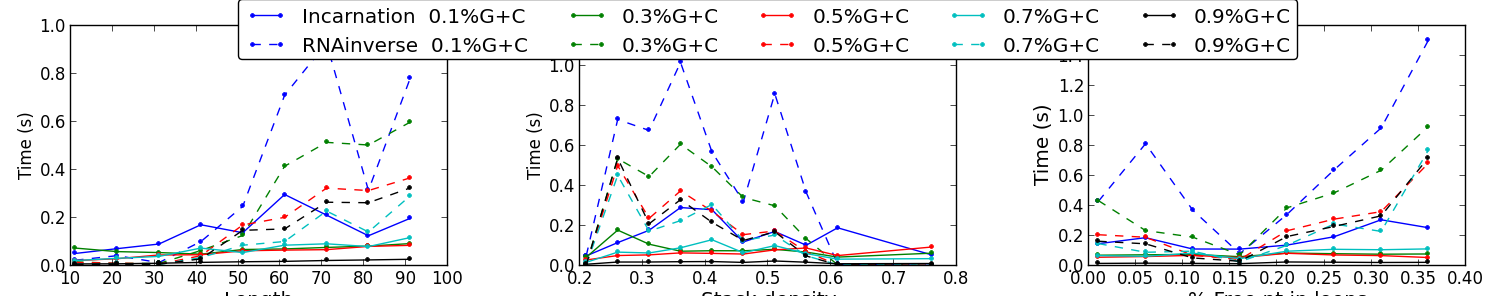
\includegraphics[width=\textwidth]{Figures/time_rnastrand_clustered_rnainverse_100samples_fix}
	\caption{Average time in seconds to generate one sequence. We explicitly show 
	the time spent by \ourprog (full line) and \texttt{RNAinverse} (dashed) for various \GCContent. The first plot is in function
	of the length of the structures. The second is in function of the stack
	density (i.e. $2\cdot\#stacks/length$) and the latter in function of 
	the proportion of free nucleotides (i.e. unpaired bases) within loops.}
	\label{fig:time}	
\end{figure}

Figure~\ref{fig:time} presents the average times spent running \ourprog and \RNAinverse to generate one sequence
with the required \GCContent. As expected, the time grows linearly
in function of the length of the structures for \ourprog.  A highly intriguing feature is the substantial decrease of the time 
required for running \RNAinverse when $15\%$ of nucleotides are unpaired in the target structure.
However, one must remain careful interpreting this observation, as the structures within this class all originate from the PDB, and are relatively small (for the complete STRAND DB, the average length is $\sim526$nts, compared to $\sim38$nts around 15\% unpaired bases).



\subsection{Dataset}
To evaluate the quality of our method, we used secondary
structures from the \RNASTRAND database~\cite{andronescu2008rna}.
Those are known secondary structure from a variety of organisms.
We considered a subset of $50$ structures selected by Levin~\emph{et al}~\cite{Levin:2012kx}, 
whose length ranges between $20$ and $100$ nucleotides. 
 To ease the visualization of results, we clustered together structures
 having similar length, stacks density and proportion of free nucleotides in loops, leading to distributions of structures shown in Figure~\ref{fig:bins}.

 \begin{figure}[ht!]
 	\centering
	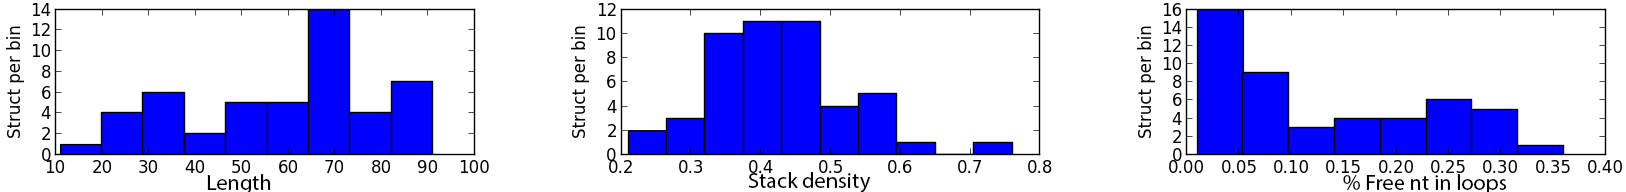
\includegraphics[width=\textwidth]{Figures/bins_distribution.png}
	\caption{Number of secondary structures per bin, according to our three clustering criteria.}
	\label{fig:bins}
 \end{figure}
 
 
\subsection{Design}
 To benchmark our method, we first started by sampling about $1000$ sequences per structure. After correcting the free nucleotides with
 \texttt{RNAinverse} we computed their MFE with \texttt{RNAfold} from the \textit{Vienna Package 2.0}~\cite{Hofacker:1994}.
 
A first criterion is the proportion of sequences accepting the target
secondary structures as their MFE. A second criterion is the number of structures
for which at least one sequence with the desired MFE was produced.
Figure~\ref{fig:mfe_struct_solved_noinverse} shows the results obtained by \ourprog for these criteria. As mentioned earlier, the high rate of failure
is due to the fact that no selection criterion is applied to
unpaired nucleotides. A local strategy is thus needed.
After processing \ourprog sequences with \RNAinverse to 
locally optimize the free nucleotides, we obtained the results 
summarized by Figure~\ref{fig:mfe_struct_solved}. We observed
that length is, in general, not a good predictor for the hardness of designing a structure. 
Instead, a high number of free nucleotides in the structure seems to be a 
good measure of its design hardness. 
 The difficulty of 
designing sequences for targets with a high number of free nucleotides 
 in loops appears clearly in the last column of Figure~\ref{fig:mfe_struct_solved}.
Even with a \GCContent of $50\%$ and more, when at least
one solution was found for almost all structures, most of the samples 
do not fold into the target. A few structures remained unsolved under
all \GCContent.


\begin{figure}[ht!]	
	\centering
	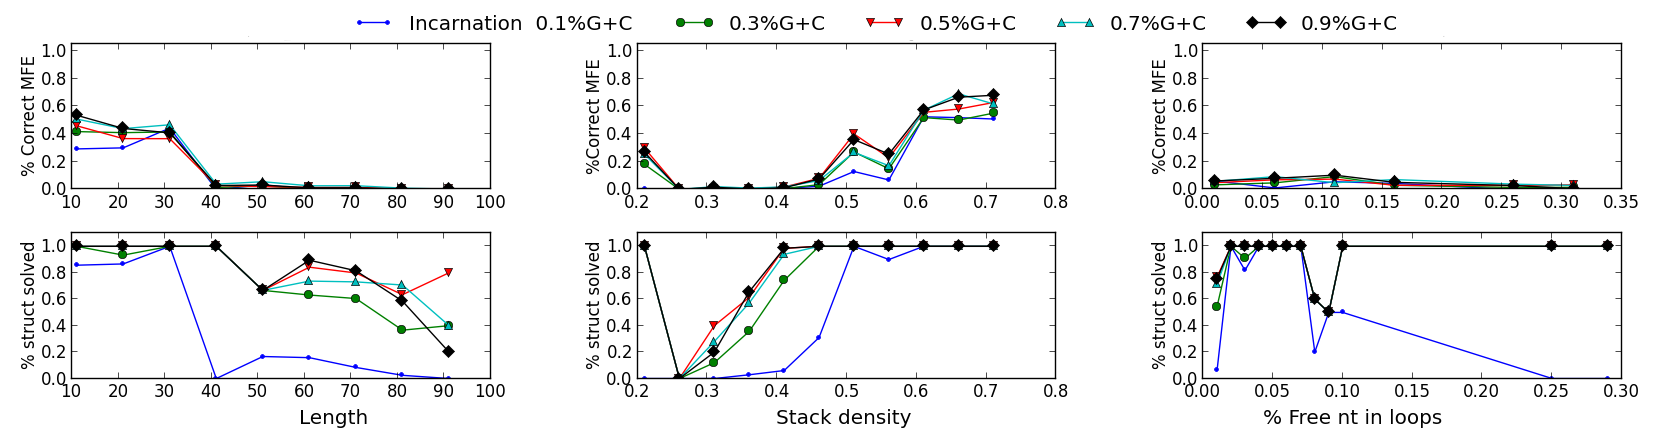
\includegraphics[width=\textwidth]{Figures/mfe_struct_solve_nornainverse.png}
	\caption{Quality of \ourprog results. The first row shows the percentage
	of sampled sequences folding into the target. The second shows the 	
	proportion	of structures for which at least one correct sequence was 
	sampled.}
	\label{fig:mfe_struct_solved_noinverse}	
\end{figure}



\begin{figure}[ht!]	
	\centering
	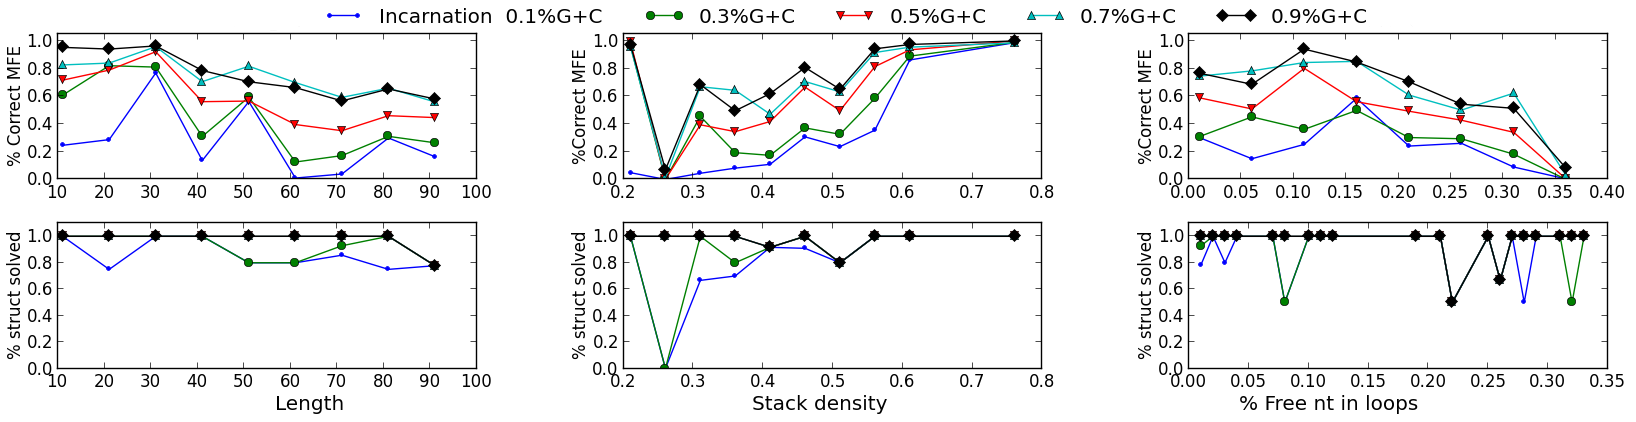
\includegraphics[width=\textwidth]{Figures/mfe_struct_solved}
	\caption{Quality of \texttt{Incarnation+RNAinverse} results. The first row shows the percentage
	of sampled sequences folding into the target. The second shows the 	
	proportion	of structures for which at least one correct sequence was 
	sampled.}
	\label{fig:mfe_struct_solved}	
\end{figure}
 
To evaluate the global quality of \ourprog sequences, we show
in Figure~\ref{fig:ss_sens} the ratio of well predicted base pairs in the
MFE structure of our sampled sequences. We can observe that, in all cases,
the hardest sequence to design are those with an extremely low \GCContent. As anticipated, those are the sequences with the weakest bonds.
We notice that the most accurate sequences yield a \GCContent
of $70\pm 10\%$. 

As discussed in Sec.~\ref{sec:implementation}, we notice a highly decreased
computational time needed to generate the sequences with $15\%$ free 
nucleotides in the loops. We remark that those structures also yield 
a much lower structural sensitivity.

\begin{figure}[ht!]
 	\centering
	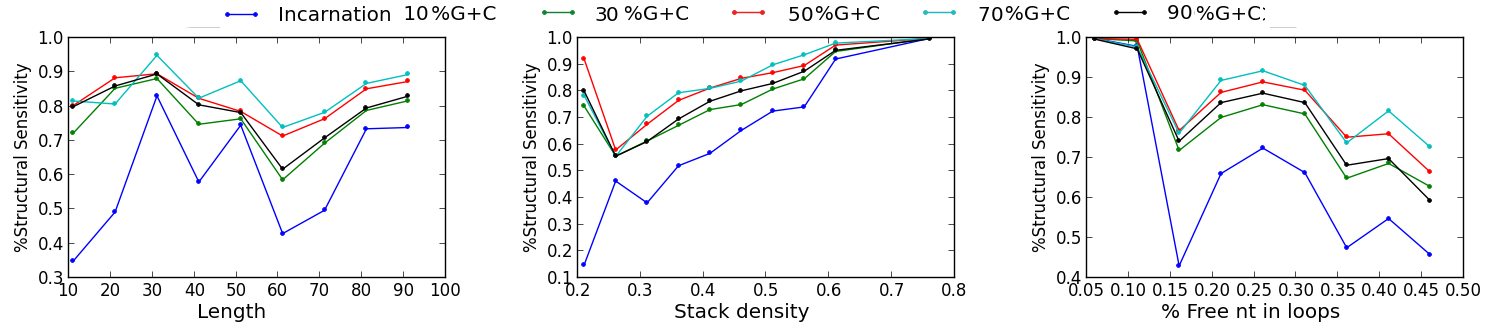
\includegraphics[scale=0.45]{Figures/rnastrand_clustered_rnainverse_100samples_struct_sens.png}
	\caption{Structural sensitivity (i.e. $\#$ well predicted base pairs / $\#$ base pairs in target) of the sampled sequences MFE. }
	\label{fig:ss_sens}	
\end{figure}


\subsection{Samples properties}

In this section, we further analyze the generated sequences that fold into the 
target structure. 

A desirable feature in sequence design, is to produce samples with a high
diversity. Figure~\ref{fig:nb_sols_entropy} shows the number of correct
solutions as their average entropy and base pair entropy, since 
\ourprog  only influences the distribution of nucleotides inside 
stacked base pairs. The most constraining factor for generating valid
 solutions seems to be  low \GCContent and the percentage of free nucleotides. 

%Our method is able to generate 

Also, a critical propertie in RNA sequence design is 
the frequency of the MFE. 
The sequence should be in its target conformation long enough to
perform the desired action. Presented in Figure~\ref{fig:freq} we see that
there is a slow decline of the frequency with the increase in size. Yet,
for an average \GCContent, the frequency stays over $10\%$ even
at size of $100$ nucleotides.


\begin{figure}[ht!]
	\centering
	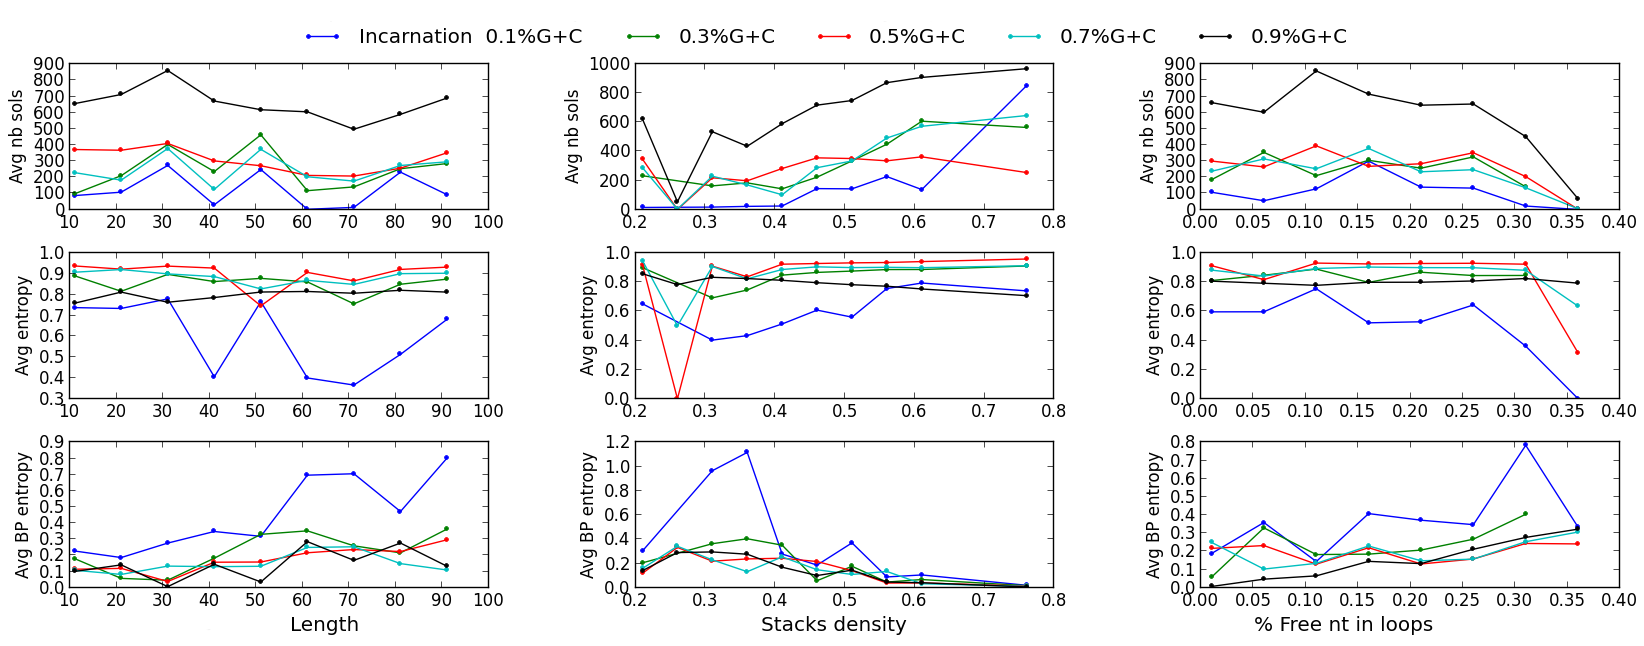
\includegraphics[width=\textwidth]{Figures/nb_sols_entropy.png}
	\caption{Number of solutions generated and their average entropy. 
	The last row presents only the entropy of the nucleotides inside base 
	pairs.}
	\label{fig:nb_sols_entropy}
\end{figure}



\begin{figure}[ht!]
	\centering
	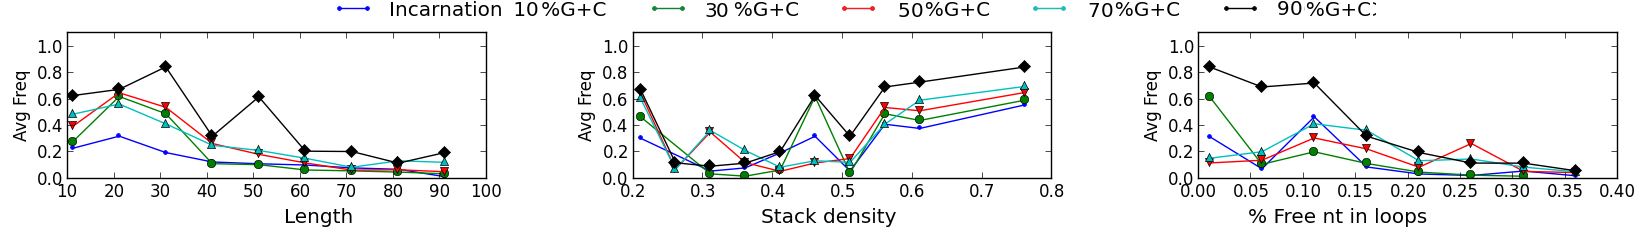
\includegraphics[width=\textwidth]{Figures/freq.png}
	\caption{Average Boltzmann probability of the MFE.}
	\label{fig:freq}
\end{figure}

\subsection{Global sampling vs Local search vs Glocal approach}


Here, we are interested in estimating the impact of the design methodology on the performances. More precisely, we aim to determine the merits of a global sampling approach (\ourprog), compared to a glocal procedure (\ourprog + \RNAinverse) and a local search methodology (\RNAinverse). 

Our results (See Fig. \ref{fig:rnainverse} in Supplementary Material) indicate that a glocal approach produces sequences that are consistently more diverse than those obtained with both {\em pure} methods alone. Furthermore, while \ourprog outperforms \RNAinverse for extreme pressures on the \GCContent, \RNAinverse produces more entropic sequences than \ourprog for the central \GCContent regime ($30\%-70\%$). 

It should be noted, however, than \RNAinverse produces sequences whose \GCContent is extremely concentrated (see Table~\ref{tab:nb_rnainv} in Supplementary Material), thereby requiring a large number of runs before producing a suitable \GCContent sequence. Therefore, a rejection algorithm based on \RNAinverse alone should not be considered a realistic solution for the design with constrained \GCContent. 

{\em Ajouter considérations Base Pair entropy: Se rappeler, que moins, c'est mieux !}




% \ourprog outperforms other strategies for non-centered . In particular, the base pair entropy as well as diversity of sequences are favorable to \ourprog. This advantage is even more striking for low targeted \GCContent{}s regimes.
%To complete this benchmark, we added the results obtained with the glocal procedure (\ourprog + \RNAinverse). We note that the results are slightly lower than those of \ourprog alone. However, we must stress that the \ourprog data consider only the sample of \ourprog already satisfying the MFE criterion. In fact \RNAinverse enable to ``correct'' a lot of sample sampled by \ourprog but without the good folding properties. Hence, our conclusion here is that the glocal approach enable us to conserve the same level of performance but to drastically improve the success rate of our methodology. 






\label{fig:rnainverse}



%!TEX root = main_ISMB.tex
\section{Conclusion}

\label{sec:conclusion}

In this article, we described a novel algorithm, \ourprog, for the RNA design problem, i.e. the design of an RNA sequence adopting a predefined secondary structure as its minimal free-energy fold.
Implementing a global sampling approach, it optimizes affinity towards the target secondary structure, while granting the user full control over the \GCContent of the resulting sequences.
This extended control does not necessarily induce additional computational demands, and we showed the linear complexity of both the preprocessing stage and the generation of candidate sequences for the design, allowing for the design of larger and more complex secondary structures in a matter of minutes on a single processor (e.g. $\sim$28 mins for 100 candidate sequences for a $\sim$1500nts 16s rRNA). We evaluated the method on a benchmark composed of target secondary structures extracted from the \RNASTRAND database. We observed good overall success rate, with the notable exception of very low targeted \GCContent ($10\%$), and a good to excellent entropy within designed candidates.
Finally, we implemented an hybrid approach, using the \RNAinverse software as a post-processing step for unpaired regions. This approach greatly increased the success rate of the method, allowing for the design of highly diverse candidates for almost all of the structures in our benchmark, while largely preserving the targeted \GCContent.

In the future, we would like to complement this study by further investigating the potential of hybrid local/global -- or {\em glocal} -- approaches.
A global sampling approach would capture the positive aspects of design, optimizing affinity towards a given structure while allowing the specification of expressive systems of constraints.
Designed sequences would serve as a seed for a restricted local approach which, by breaking unwanted symmetries, would perform the negative part of the design, 
while ideally maintaining obedience to the constraints. Another perspective of this work is the incorporation of the full Turner energy model, which should in principle yield better designs for unpaired regions.

%!TEX root = main_ISMB.tex
%\section{Acknowledgments}
\label{sec:acknowledgments}


\newpage

\bibliographystyle{natbib}
\bibliography{RNApyro}

\newpage

%!TEX root = main_ISMB.tex
\section{Supplementary data}

\subsection{Benchmark \ourprog+\RNAinverse}
To emphasize the usefulness of processing \ourprog sequences with \RNAinverse, we present the number
of structures for which at least one sequence was generated with the desired MFE in Figure.~\ref{fig:nb_sols}

\begin{figure*}[ht!]
  \centering
  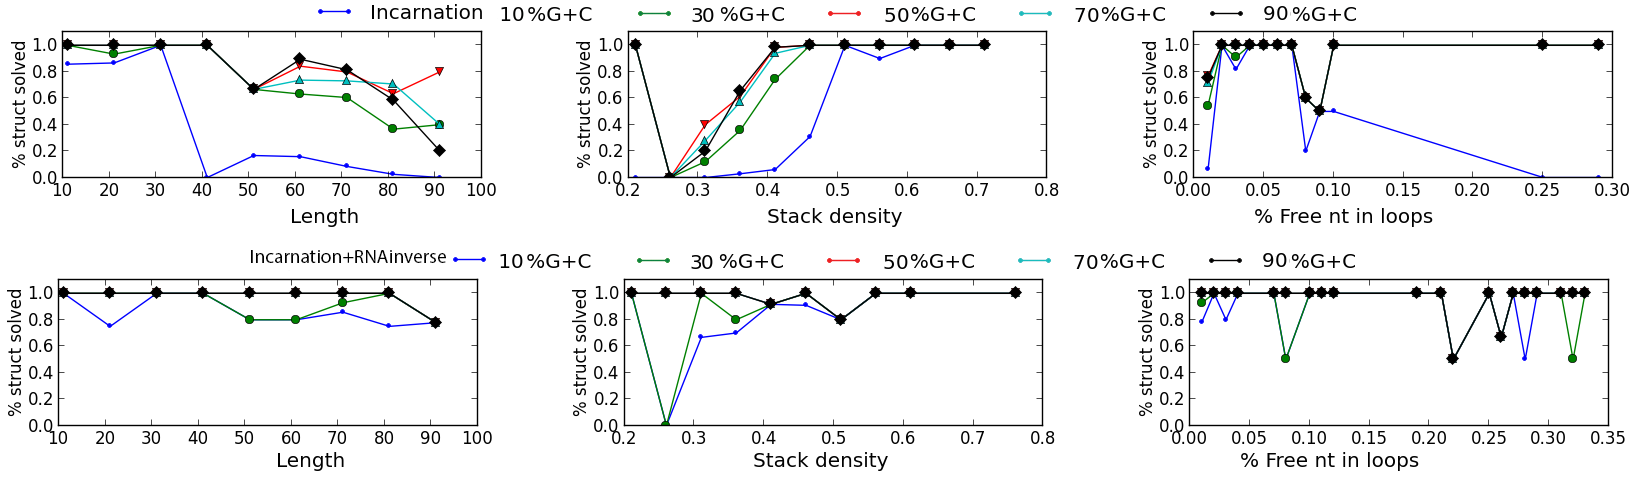
\includegraphics[width=\textwidth]{Figures/struct_solved_vsrnainverse.png}
  \caption{The first row shows the number of structures for which one generated sequence has the 
  structure as MFE when only using \ourprog. The second row shows when we process \ourprog results with \RNAinverse.}
  \label{fig:nb_sols}
\end{figure*}


\subsection{Benchmark \ourprog vs \RNASSD}
%Using the same dataset of $50$ structures, we generated $100$ samples
%per structure %with \RNAinverse. They yield for most parameters
%a high entropy.
%Table.~\ref{tab:nb_rnainv} contains the number of samples with a given \GCContent generated
%with  \RNAinverse, \INFORNA, \NUPACK and \frankenstein. They have a highly concentrated distribution of \GC content showing one of theirs major deficiencies. We present in Fig.~\ref{fig:gcdist} those distributions.

%\begin{figure}[ht]
%  \begin{center}
%    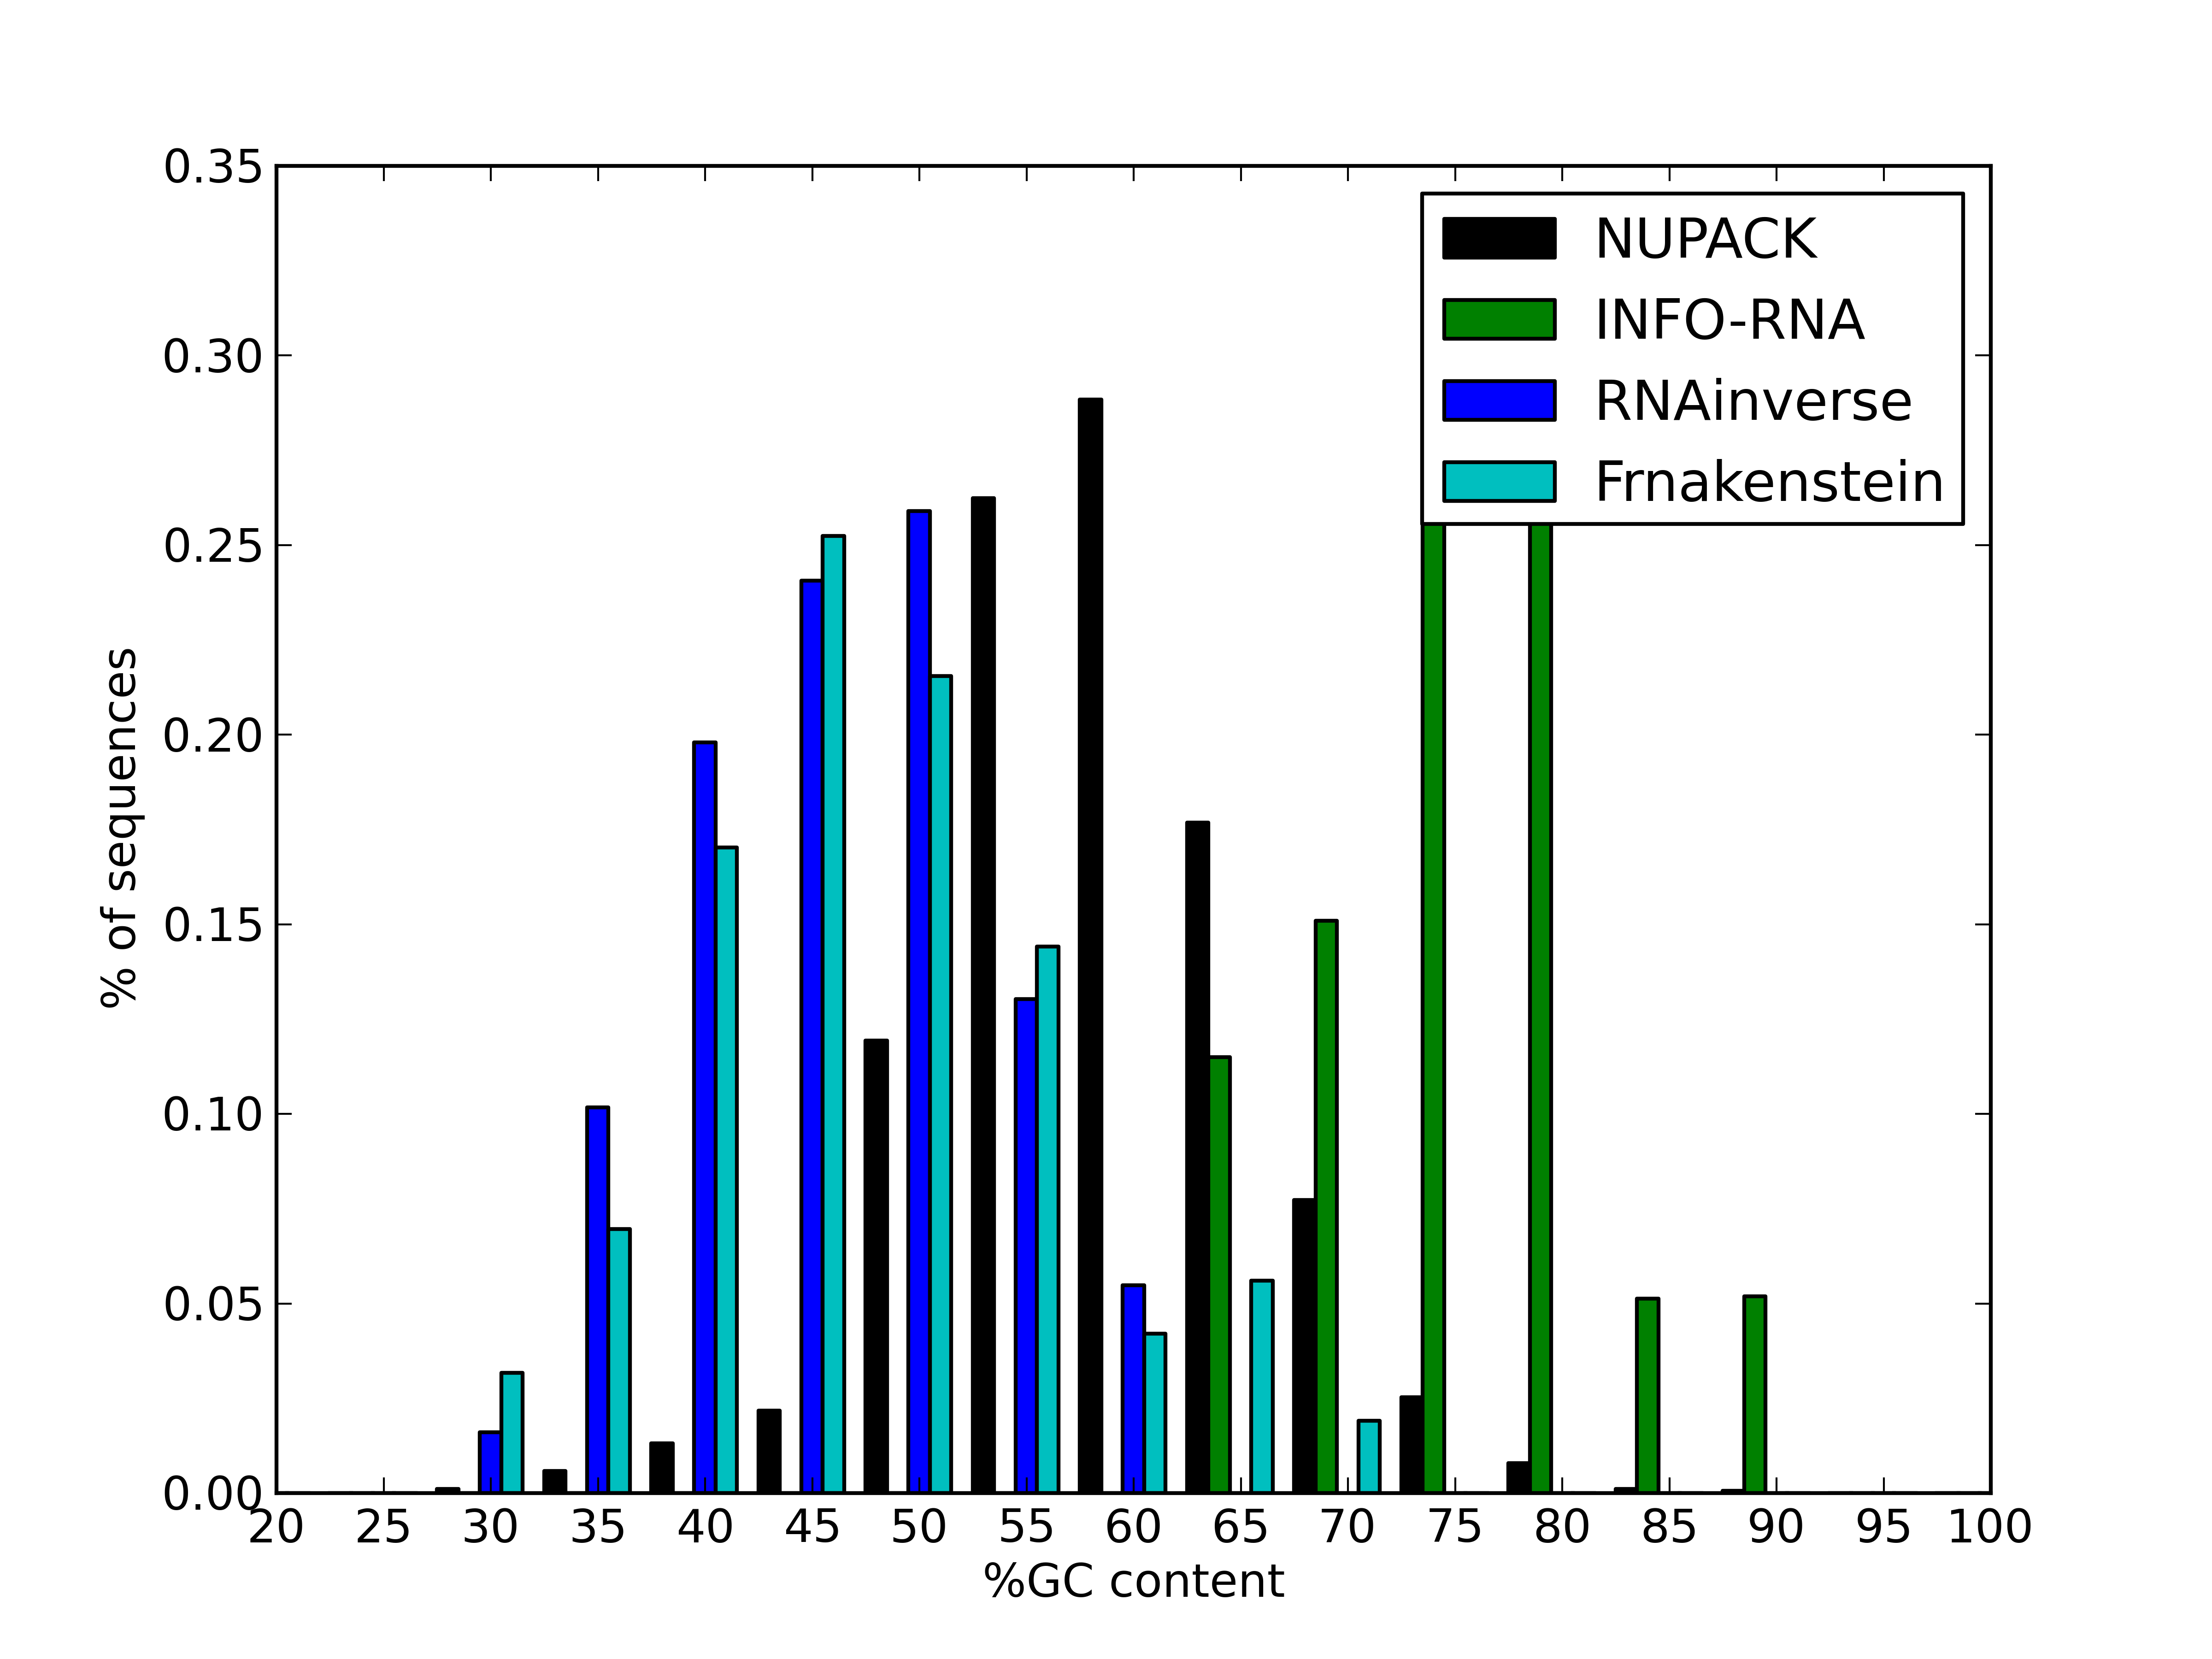
\includegraphics[width=0.5\textwidth]{Figures/histograme_5_gc_distribution_nornaexinv.png}
%  \end{center}
%  \caption{Overall \GCContent distribution for sequences designed using \RNAinverse, \INFORNA, \NUPACK and \frankenstein folding in the desired structure.}
%  \label{fig:gcdist}
%\end{figure}

 For all structures that have been solved 
by the three methods, only \RNASSD, only \texttt{Incarnation} and
\texttt{Incarnation} followed by \RNAinverse, 
we present for different concentration of \GCContent the average sequence identity in Figure.~\ref{fig:identity_50_70_90}
%the average sample entropy and the average base pairs entropy in Figure.~\ref{fig:rnainverse}.

\begin{figure*}[ht!]
  \centering
  \includegraphics[width=\textwidth]{Figures/seq_identity_50_70_90.png}
  \caption{Sequence identity by average \GCContent of $50$, $70$ and $90\%$ for \ourprog,\ourprog+\RNAinverse and \RNASSD.}
  \label{fig:identity_50_70_90}
\end{figure*}
%\begin{table}[h!]
%	\begin{center}
%		\begin{tabular}{|c|ccccc|}
%		\hline
%		Target \GCContent & 10 & 30 & 50 & 70 & 90\\ \hline
%   $\#$\RNAinverse samples& 11 & 437 & 3362 & 1155 & 35\\ \hline
%		\end{tabular}
%	\end{center}
%  \caption{Overall \GCContent distribution for sequences designed using \RNAinverse.}
%	\label{tab:nb_rnainv}
%\end{table}




%\begin{figure*}[ht!]
%	\centering
	%\hspace{-5em}
%	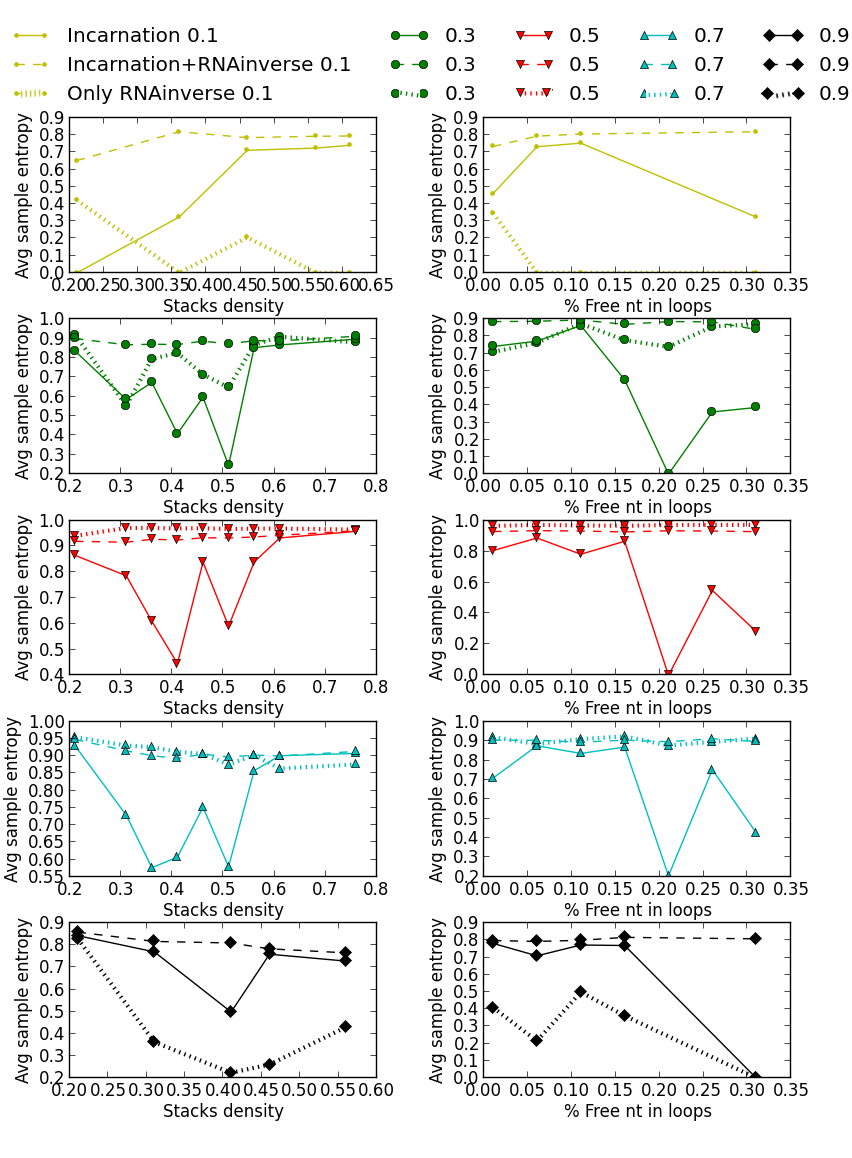
\includegraphics[width=0.5\textwidth]{Figures/RNAinverse_data_100.png}
%	\caption{Entropy and \GCContent  for structures solved by
%	the 3 methods.}
%	\label{fig:rnainverse}
%\end{figure*}
%{\em Récupérer Base-pair entropy}


%The same analysis but only for structures solved by \texttt{Incarnation}
%and \texttt{Incarnation} followed by \RNAinverse, is presented in 
%Fig.~\ref{fig:inc_rnainv}
%
%\begin{figure}
%	\centering
%	\includegraphics{}
%	\caption{Entropy and \texttt{C+G} content for structures solved by
%	the \texttt{Incarnation} and \texttt{Incarnation}$+$\RNAinverse.}
%	\label{fig:inc_rnainv}
%\end{figure}

\subsection{Limited impact on \GC of local-search postprocessing of \ourprog output}
Since local search approaches tend to experience a bias towards \GC{}-rich regions, it could be expected that our glocal approach, by postprocessing unpaired regions using a local search algorithm, would suffer from such a drift.
However, as summarized in Table~\ref{table:impact_on_gc}, we observed that the local search heuristic used to design nucleotides in loop regions has a very limited impact on the \GCContent. For each class of \GCContent, we reported the observed \GCContent in the sequence initially generated by \ourprog, and the observed \GCContent after the \RNAinverse postprocessing (as defined in Section \ref{subsec:glocal_method}). Our results show that the \GCContent is relatively well conserved (less than 6\% variation), with a general tendency of the postprocessing step to bring the \GCContent back to 50\%. 

\begin{table}[h!]
\begin{center}
\resizebox{0.5\textwidth}{!}{
\begin{tabular}{|c|c|c|}
\hline
\multirow{3}{*}{Target \GCContent (\%)}& \multicolumn{2}{c|}{\GCContent (\%) of designed sequences}\\ \cline{2-3}
 & \ourprog & \ourprog + \RNAinverse\\
 & (Global) & ({Glocal}) \\
\hline
10\% & 15\% & 21\% \quad $\nearrow 6\%$\\
30\% & 30\% & 33\% \quad $\nearrow 3\%$\\
50\% & 48\% & 49\% \quad $\nearrow 1\%$\\
70\% & 71\% & 69\% \quad $\searrow 2\%$\\
90\% & 83\% & 78\% \quad $\searrow 5\%$\\
\hline
\end{tabular}
}
\end{center}
\caption{Observed \GCContent of solutions returned by \ourprog (2nd column) and after the application of the local search postprocessing (3rd column).}
\label{table:impact_on_gc}
\end{table}


\end{document}  
